\NeedsTeXFormat{LaTeX2e}
%thesis document class
\documentclass[12pt,twoside,a4paper]{report}

%_________________________________preamble________________________________________

%http://www.howtotex.com/packages/9-essential-latex-packages-everyone-should-use/

%https://www.ctan.org/pkg/nag
\RequirePackage[l2tabu, orthodox]{nag}
%
\usepackage[utf8]{inputenc}

%https://www.ctan.org/pkg/indentfirst?lang=en
\usepackage{indentfirst}

%https://www.ctan.org/pkg/microtype
\usepackage{microtype}

%https://www.ctan.org/pkg/setspace?lang=en
\usepackage{setspace}

%https://www.ctan.org/pkg/amsmath
\usepackage{amsmath, amssymb, amsthm}

%https://www.ctan.org/pkg/siunitx
\usepackage{siunitx}

%https://www.ctan.org/pkg/geometry
\usepackage[a4paper]{geometry}

%https://www.ctan.org/pkg/fancybox
\usepackage{fancybox}

%https://www.ctan.org/pkg/listings
\usepackage{listings}

\usepackage{color}
 
\definecolor{codegreen}{rgb}{0,0.6,0}
\definecolor{codegray}{rgb}{0.5,0.5,0.5}
\definecolor{codepurple}{rgb}{0.58,0,0.82}
\definecolor{backcolour}{rgb}{0.95,0.95,0.92}

\lstdefinestyle{mystyle}{
    backgroundcolor=\color{backcolour},   
    commentstyle=\color{codegreen},
    keywordstyle=\color{magenta},
    numberstyle=\tiny\color{codegray},
    stringstyle=\color{codepurple},
    basicstyle=\footnotesize,
    breakatwhitespace=false,         
    breaklines=true,                 
    captionpos=b,                    
    keepspaces=true,                 
    numbers=left,                    
    numbersep=5pt,                  
    showspaces=false,                
    showstringspaces=false,
    showtabs=false,                  
    tabsize=2
}
 
\lstset{style=mystyle}

%https://www.ctan.org/pkg/url?lang=en
\usepackage{url}

%https://www.ctan.org/pkg/graphicx?lang=en
\usepackage{graphicx}

%https://www.ctan.org/pkg/array?lang=en
\usepackage{array}

%https://www.ctan.org/pkg/fancyhdr?lang=en
\usepackage{fancyhdr}

%https://www.ctan.org/pkg/booktabs
\usepackage{booktabs}

%http://www.tug.dk/FontCatalogue/lmodern/
\usepackage{lmodern}
\usepackage[T1]{fontenc}

%https://www.ctan.org/pkg/hyperref?lang=en
\usepackage{hyperref}
% pdf settings assures outlines being created
\hypersetup{
	pdftitle={Play With Scala},
    pdfauthor={Martin Zuber},
    pdfsubject={Functional Programming in Scala},
    pdfkeywords={functional programming, scala},
    bookmarksnumbered=true,     
    bookmarksopen=true,         
    bookmarksopenlevel=1,       
    colorlinks=true,            
    pdfstartview=Fit,           
    pdfpagemode=UseOutlines,
    pdfpagelayout=TwoPageRight
}

%https://www.ctan.org/pkg/cleveref
\usepackage{cleveref}

\graphicspath{ {figures/} }

%paragraph formatting from thesis guidelines
\setlength{\textheight}{9in}
\setlength{\textwidth}{6in}
\setlength{\oddsidemargin}{.25in}
\setlength{\topmargin}{-.5in}
\setlength{\parindent}{2em}
\setlength{\parskip}{1em}
\setstretch{1.6667}
\hyphenation{itself}

\pagestyle{fancy}
\fancyhf{}
\rhead{Martin Zuber}
\lhead{BSc in Computing}
\cfoot{Page \thepage}

%__________________________________content_____________________________________

\title{Play with Scala\\Functional Programming Course}
\author{Martin Zuber, B00066378 \\ Project Supervisor:  Luke Raeside}
\date{\today}

\begin{document}

\pagenumbering{roman}
\maketitle
\newpage

%_______________________________chapter_______________________________________
\chapter*{Declaration}
I hereby certify that this material, which I now submit for assessment on the programme of study leading to the award of Degree of Honours B.Sc. in Computer Science in the Institute of Technology Blanchardstown, is entirely my own work except where otherwise stated, and has not been submitted for assessment for an academic purpose at this or any other academic institution other than in partial fulfilment of the requirements of that stated above.

%_______________________________chapter_______________________________________
\chapter*{Acknowledgements}
In performing my assignment, I had to take the help and guideline of some respected persons, who deserve my greatest gratitude. The completion of this assignment gives me much Pleasure. I would like to show my gratitude to the project supervisor Dr Luke Raeside, Institute of Technology, Blanchardstown for giving me good guidelines for the thesis throughout numerous consultations. I would also like to expand my deepest gratitude to all those who have directly and indirectly guided me in writing this thesis, especially Dr Markus Hofmann.

%_______________________________chapter_______________________________________
\chapter*{Abstract}
This paper is dedicated to computer programming with the focus on programming styles found in modern application development. The idea for the project came to life when I, the author and computer science student realized there are programming styles other than imperative and object-oriented programming. Namely functional programming paradigm. The lack of a study material dedicated to the functional programming withing the ITB Computer Science course curriculum and my curiosity toward the subject I decided to research and to learn the paradigm. I decided to use the course final project as the vehicle for this endeavour.\par
This paper is discussing functional programming paradigm with Scala programming language and web application development process using Play! Framework. The target audience is any computer science student with knowledge of a programming language such as Java and with an understanding of some of the object-oriented programming principles such as inheritance and polymorphisms.\par
Please keep in mind that I had no knowledge of a functional programming, Scala programming language or Play! framework prior to this endeavour. This document is basically a report of a student learning basics of these concepts and tools. I can only hope that I would be able to communicate clearly what I learn and in this document's usefulness.

\listoffigures
\listoftables
\tableofcontents{}
\pagenumbering{arabic}

%_______________________________chapter_______________________________________
\chapter{Introduction}\label{1}
\section{Introduction}\label{1.1}
In the world of multi-core processors, distributed systems and big data, we are witnessing a paradigm shift in the computational model used within application development industry. It's a shift from imperative programming style toward declarative programming and the rise of the functional programming languages \cite{1}. JVM ecosystem is no exception.\par
Even though Java being still most used JVM language and one of the most used programming languages overall, JVM languages such as Scala, Groovy and Clojure are getting more popular every day. Java itself with recent SE 8 update brought limited support for functional programming as well.\par
Scala programming language \cite{2} is getting a big momentum in the last few years \cite{3}. Companies such as Twitter or LinkedIn \cite{4} had switched to Scala for their web applications development. Scala is being a big player in the realm of Reactive programming, Distributed Systems and Big Data \cite{5}.
\subsection{Some of the reasons for Scala success}\label{1.1.1}
\begin{itemize}\itemsep1pt \parskip0pt \parsep0pt
\item Scala is elegant, scalable, purely object-oriented and fully functional programming language with the performance comparable to Java.
\item Scala compiles to JVM byte code .class files which mean that Scala is fully compatible with existing Java libraries or frameworks and vice versa. Mixed Java / Scala projects are quite common.
\item Existence of powerful, open source and award-winning frameworks \cite{6}, toolkits, platforms and build tools written in Scala, such as Akka, Spark, Play, SBT \cite{7}.
\end{itemize}
\section{Aims and Objectives}\label{1.2}
The idea is to develop a web application for a computer science student who would like to learn Scala programming language and functional programming paradigm. The application will be developed using MVC Play! Framework. I decided to work on this project for the following reasons:
\begin{itemize}\itemsep1pt \parskip0pt \parsep0pt
\item Strong personal interest in functional programming.
\item Lack of modules dedicated to functional programming in ITB curriculum.
\item Solid background in Java platform.
\item Desire to pursue a Java / Scala development professional career.
\end{itemize}
\subsection{Web Application Proposed functionality}\label{1.2.1}
\begin{itemize}\itemsep1pt \parskip0pt \parsep0pt
\item A student can register the account.
\item The authenticated student will gain access to the functional programming with Scala lectures and exercises.
\item The student will have access to Scala interpreter where he could carry out coding exercises.
\item The student will be able to communicate with other users through a chat window or other messaging functionality.
\item The student will be able to upload the files, for example an exercise solution.
\end{itemize}
\section{Main Research Questions}\label{1.3}
\begin{itemize}\itemsep1pt \parskip0pt \parsep0pt
\item What exactly is functional programming and what benefits does it bring to application development?
\item In what ways Scala supports the paradigm?
\item What exactly is Play framework and what kind of applications we can develop with it?
\item What are the advantages and disadvantages of Play framework in terms of productivity, performance and scalability and in comparison to other frameworks?
\end{itemize}
\section{Justifications / Benefits}\label{1.4}
As mentioned earlier, there is not a module dedicated to functional programming in ITB Computer Science course curriculum. I can actually claim that there is no mention of this programming style in any module overall and the paradigm is totally ignored by the curriculum. In comparison, there are 8 networking modules delivered to students over the course duration. In my opinion, this makes the course unbalanced and creates an 'educational gap' in the curriculum. Personally, I feel that the topic belongs to the course curriculum and it is the natural progression from object-oriented programming and design patterns which had strong coverage in the third year of the course.\par
\textbullet \textbf{ Filling the 'educational gap' in the Computer Science course curriculum by creating learning web resource.}\par
The preliminary research on the current state of the application development industry is suggesting that fluency in a functional programming language is a really valuable skill for any developer to possess right now. Developers able to code using languages such as Scala, Clojure, F\# or Lisp dialects are in demand. Reasoning about the functional programs requires different ‘mind-set’ or ‘thought processes’ in comparison with object-oriented programming. Even if one would never use purely functional programming professionally, understanding of the concepts will make one a better programmer overall and give one deeper insight into other programming styles.\par
\textbullet \textbf{ Acquiring valuable skills and deeper insides into different programming paradigms and design patterns.}\par
Also, Scala seems to be very elegant language and takes the good design ideas from many other programming languages. The language was designed with the scalability of the syntax taken in the consideration, which allows the language to 'shape-shift' towards the needs of its users. In my opinion, the Scala programming language would be the right tool for me to learn functional programming paradigm.\par
\textbullet \textbf{ Learning Scala programming language and Java Virtual Machine (JVM).}\par
Even though learning functional programming with Scala is the main aim of this project, the additional work will be carried out by exploring Play framework and developing the web application. The preliminary research suggests the framework is a powerful tool for rapid web development. Play seems to be heavily inspired by Ruby on Rails. It supports reactive web application development and seems to be a cleaner alternative to legacy Java Enterprise stack \cite{8}.\par
\textbullet \textbf{ Building valuable skill set in contemporary web application development.}
\section{Feasibility}\label{1.5}
\textbf{Project requirements}
\begin{itemize}\itemsep1pt \parskip0pt \parsep0pt
\item Access to relevant study material and tutorials dedicated to Scala programming language and Play. There is no material available in ITB library, but there is a number of books published and available over the internet. \textit{Estimated cost is 100 euros.}
\item Access to personal computer. I'm the owner of the laptop computer, which should serve as the project workstation without too many constraints. Additional research must be done to decide on the operating system and other tools. Using free software is most desired.\textit{Estimated cost is 0 euros.}
\item Access to the internet, deployment, DNS and versioning control services, printer and thesis binding.\textit{ Estimated cost is 300 euro.}
\item At least 14 hours per week to carry out the project related work for the whole project duration. This estimation is based on personal experience I gained by working on two academic projects during my studies and on experience working on a research project as part of the summer internship.
\end{itemize}
In my opinion, all the requirements could be met to assure this project feasibility with the minimal cost associated. With proper planning, use of the personal assets and free software when possible, I should be able to meet the project goals within the given time scale.
\section{Proposed Methodologies}\label{1.6}
\subsection{Literature Review}\label{1.6.1}
The first step is to carry out the research on functional programming \cite{9}, Scala programming language \cite{10}, MVC design pattern and Play Framework \cite{11}. I'm planning to use dedicated books I acquired recently, plus online tutorials and blogs. I will analyze, summarize, and carry out the coding tutorials. The thorough literature review at the beginning should lay a foundation for following web application development. I will continue to research relevant materials for the whole duration of the project.
\subsection{The Web Application Development}\label{1.6.2}
The real challenge lies in the fact that I have a little experience developing web applications using MVC framework and no skills in technologies I decided to use during this project. I have only general ideas how to design such an application. Only layers I can design reasonably well in advance are the database relations and user interface.\par
Therefore, I must approach this problem using some kind of adaptive methodology and avoid 'a big design in advance' approach. I would argue that Prototyping SDLC is the best methodology to carry out the development. In this model, the developer basically re-analyzes, re-designs, re-implements and re-test application prototype until the product is accepted by the client.
\begin{figure}[!ht]
	\centering
		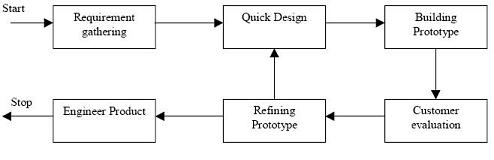
\includegraphics[width=1\textwidth, totalheight=6cm]{prototyping}
	\caption{\textit{Prototyping SDLC diagram}}
	\label{f1.1}
\end{figure}
Instead of creating 'a big design in advance', prototyping methodology is allowing the developer to change the design with each iteration of the design / development / evaluation / refining circle. I should expect major changes in design based on my lack of experience in web development and technologies I decided to use. The prototyping methodology will allow me to have a simple, but functioning prototype reasonably early. As more insights are acquired from the research, the prototype can be re-designed to implement additional functionality or re-evaluate the design.
\section{Project Plan}\label{1.7}
\textbf{Work Breakdown Structure (WBS)}
\begin{enumerate}
\item \textbf{Research.}
	\begin{enumerate}\itemsep1pt \parskip0pt \parsep0pt
	\item Research on Scala programming language design ideas and syntax, MVC design pattern, Play framework, user interface and database design.
	\item Literature Review of papers dedicated to the functional programming paradigm and test driven rapid web application development with Play.
	\item Building development platform.
	\end{enumerate}
\item \textbf{Front-End design.}
	\begin{enumerate}\itemsep1pt \parskip0pt \parsep0pt
	\item Creating wire-frame design for new view.
	\item Constructing the view.
	\end{enumerate}
\item \textbf{Database Design.}
	\begin{enumerate}\itemsep1pt \parskip0pt \parsep0pt
	\item Adding the database entity for new view.
	\item Designing the relationships with existing entities.
	\end{enumerate}
\item \textbf{Prototype Development.}
	\begin{enumerate}\itemsep1pt \parskip0pt \parsep0pt
	\item Creating the controller object.
	\item Creating unit tests.
	\item Implementing method bodies using test driven development methodology.
	\item Repeating the steps 1, 2, 3 with additional functionality until the final product is build.
	\end{enumerate}
\item \textbf{Quality Assurance.}
	\begin{enumerate}\itemsep1pt \parskip0pt \parsep0pt
	\item Performing integration tests of the whole MVC pipeline.
	\item Performing user tests.
	\end{enumerate}
\item \textbf{Post Implementation Maintenance.}
	\begin{enumerate}\itemsep1pt \parskip0pt \parsep0pt
	\item Making prototype production ready and deploying the prototype.
	\item Monitoring deployed application and adding more content.
	\item Adding content to the application.
	\item Working on project Report.
	\item Repeating steps 5.(a), 5.(b), 6.(a), 6.(b), 6.(c), 6.(d)
	\item Report Binding.
	\end{enumerate}
\end{enumerate}
\begin{figure}[!ht]
	\centering
		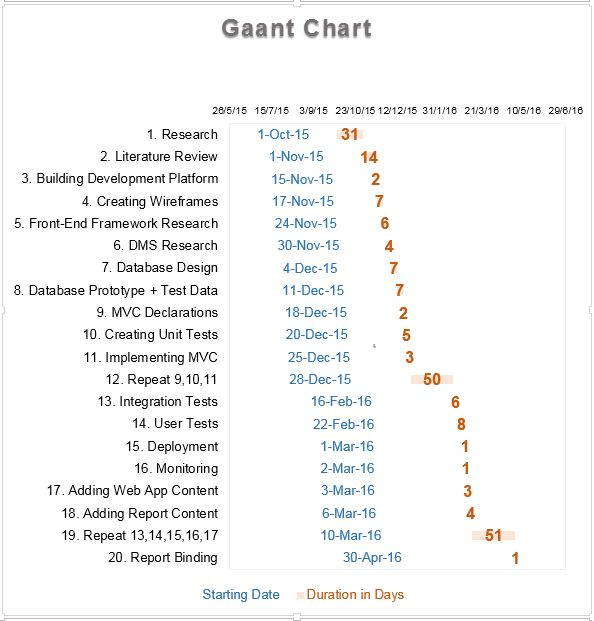
\includegraphics[width=1\textwidth,totalheight=10cm]{gaant}
	\caption{\textit{Gaant Chart}}
	\label{f1.2}
\end{figure}
\section{Expected Results}\label{1.8}
The project would be considered successful if it would meet at least two following criteria and goals. In the case of three or more goals accomplished I would consider project outcome to be very successful.
\begin{enumerate}\itemsep1pt \parskip0pt \parsep0pt
\item The gain in Scala coding skills and creation of enough learning material content for Scala course web application.
\item The comprehensive research on the functional programming paradigm and design patterns performed and gained the ability to code in the declarative style.
\item The delivery of fully functioning prototype of Scala course learning web application.
\item The acquisition of skill-set in rapid web development using Play framework.
\end{enumerate}
\section{Conclusion}\label{1.9}
At the end of this project, I will hopefully introduce some of Scala dedicated learning material in the form of an interactive web application. It can be used in a fictional course module for a fictional college. The application main purpose is to promote the interest in Scala programming language and functional programming paradigm. Especially on the personal level. After three years of my studies with ITB, I didn't learn anything about functional programming. I chose this project so I can gain a knowledge and skills which are really missing in my skill-set and which could prove very useful in the future. I hope as a fourth year student I am ready to face this challenge.\par
This research project will not contribute at all to the discipline area. Maybe only in a sense that it will hopefully bring one more student with the passion for programming languages to the functional programming paradigm. And maybe if other students or lecturers will see how elegant and declarative functional programming really is, the contribution could be a bit more significant.

%_______________________________chapter_______________________________________
\chapter{Literature Review}\label{2}
\section{Introduction}\label{2.1}
Computer programming is a fascinating and vast subject to study. Programming languages began as an attempt to translate the human language and the way of human thinking into the language of a computer.\par
The idea was to make it easier, more efficient for programmers to write the programs. With the evolution of computers, as the problems to solve became more complex, the programs became larger and more sophisticated. The programming languages quickly evolved into the forms commonly referred to as high-level programming languages. In these forms, the programming languages are hiding the internal hardware details and offer a higher level of abstractions allowing programmers to write the programs using familiar terms with an ability to model real life objects.\par
The purpose of this paper is to review some of the studies dedicated to concepts and design ideas behind the high-level programming languages. The research done in this field is immense. It is out of the scope of this paper to cover every concept,paradigm, or language and rather study some of the most important concepts in general. Then I will continue to study research papers dedicated to two most popular paradigms - object-oriented and functional programming. I will try to identify and discuss their key concepts, strength, and weaknesses and outline their history in short. I chose reading materials with a secondary intention to lay down a foundation for further studies toward a deeper understanding of the paradigms and transitions between them.
\section{General Concepts}\label{2.2}
In \emph{The Conception, Evolution, and Application of Functional Programming Languages}\cite{12} author defined a programming paradigm as an approach to a computer programming based on a coherent set of principles or a mathematical theory. The purpose for a paradigm existence is to solve a specific type of a problem. Each paradigm consists of a number of concepts. Any programming language can support one or more paradigms and the language which support more than one paradigm is called the multi-paradigm programming language. Different languages can interpret the concepts of a paradigm differently and often the implementations differ from language to language as well. The author listed around 30 useful programming paradigms implemented by modern programming languages.
\begin{figure}[!hb]
	\centering
		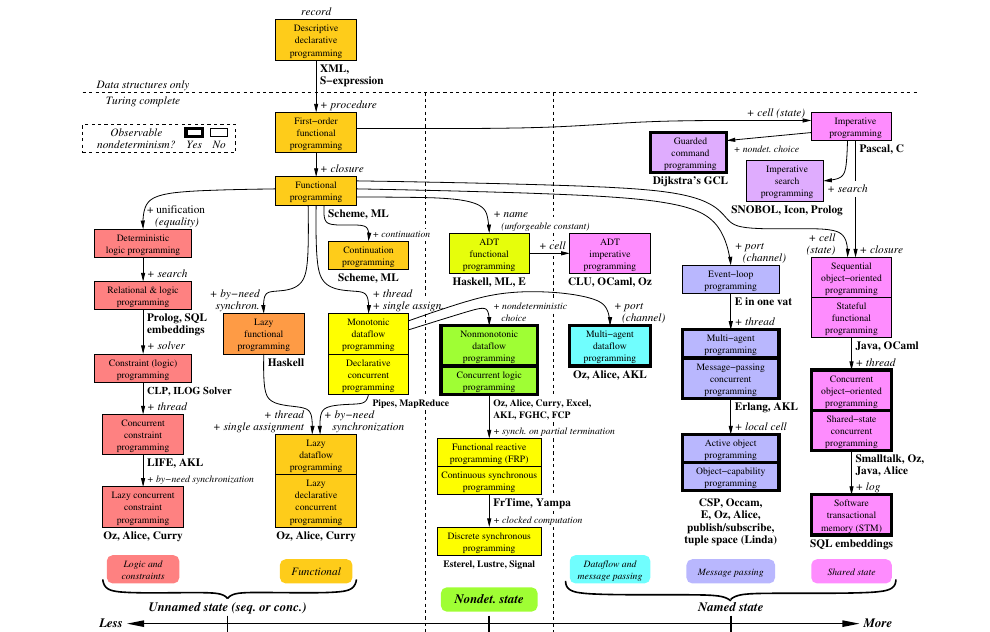
\includegraphics[width=1\textwidth,totalheight=12cm]{taxonomyDiagram}
	\caption{\textit{Taxonomy of programming paradigms (Van Roy, page 15)}}
	\label{f2.1}
\end{figure}
Author then identified the two most important properties which differentiate the programming paradigms:
\begin{enumerate}
\item \textit{Observable nondeterminism} is when a program is not completely determined by its specification. In other words with each execution the same program can produce different results. Observable nondeterminism is caused by the run-time scheduler and its usual effect is a race condition, which is often used as the synonym for Observable nondeterminism.
\item \textit{Named state} is an ability of a program to store values in time. This ability is highly influenced by the paradigm it contains it.
\end{enumerate}
As mentioned before, the programming paradigms are based on a number of concepts. Author identified four most important programming concepts:
\begin{enumerate}\itemsep1pt \parskip0pt \parsep0pt
\item \textbf{Record} is a data-structure. Every programming language should be able to work with records. Arrays, lists, strings, trees and hash tables are derived from records.
\item \textbf{Lexically scoped closure} is a record storing a function together with an environment referenced at the time of that function definition. Closure is a very powerful concept and constructs such as \textit{objects} or \textit{control structures} have been implemented with closures in many programming languages.
\item \textbf{Independence} is when a program is constructed from independent parts. When parts don’t interact with each other we call them \textit{concurrent}. When an order of the execution is given, the parts are called sequential. The interaction between the parts is called communication. Author recognizes three levels of concurrency:
    \begin{enumerate}\itemsep1pt \parskip0pt \parsep0pt
    \item \textit{Distributed system,} where concurrent activities (parts) are computers.
    \item \textit{Operating system,} where concurrent activities are processes. This level of concurrency is often called competitive concurrency because the processes are competing for access to system resources.
    \item \textit{Inter Process,} where concurrent activities are threads. This level of concurrency is called \textit{cooperative concurrency} because the threads are cooperating to achieve the result of the process. There are two popular paradigms for inter process concurrency: \textit{Shared state concurrency}, where shared data are accessed by threads using control structures called \textit{monitors}. The second approach is \textit{message-passing concurrency}, where threads are communicating by sending messages to each other.
    \end{enumerate}
\item \textbf{Named State} Author showed how named state could be implemented with a help of internal memory (variables).
\end{enumerate}
\section{Specific Characteristics}\label{2.3}
\subsection{Object Oriented Programming}\label{2.3.1}
In \emph{A Survey of Object Oriented Programming Languages}\cite{13} authors argued that consensus on what key concepts of Object Oriented Programming still don't exist. They argue that the most fundamental concepts behind the paradigm are as follows:
\begin{enumerate}\itemsep1pt \parskip0pt \parsep0pt
\item \textbf{Class} is a mechanism which group together attributes and methods with common properties. The class describes the run-time behavior of the objects instantiated from it. The well-designed class would have an immutable interface clients can use.
\item \textbf{Abstraction} is a simplified view of reality. Presented to clients by class methods and attributes.
\item \textbf{Inheritance} is a mechanism to create hierarchical class designs by creating a child class of the original class. A child class inherits the parent class behavior which can be then extended. Multiple inheritance allows for a class to inherit the behavior of multiple parent classes.
\item \textbf{Encapsulation} is hiding implementation details within the class. Only the interface is presented to the
clients.
\item \textbf{Polymorphism} is allowing to similar looking structures to handle a variety of objects.
\end{enumerate}
Authors then discussed inheritance and polymorphism in detail. I will outline the important key points.
\subsubsection{Inheritance}
As mentioned earlier the inheritance brings the hierarchical relationship into the class model. Authors pointed out that many languages define the most generic class that is an ancestor for all the classes in the language. This applies that any class can be downcast to the pointer of that ancestor. Authors pointed out that inheritance provides the ability to represent an \textit{“is a”} relationship in software. This relationship can be violated if child class extends the inherited code the way which changes the code semantics. It is the reason for the inheritance to be used with caution.\par
Inheritance also allows to represent generalization /specialization relationships with method redefinition. This functionality is breaking the encapsulation because the child class has access to parent class hidden methods and attributes. This problem can be addressed by defining a well-defined interface for the descendants. Authors argued that literary every object-oriented language provides the ability for a child class to invoke parent class methods. Even those methods which were redefined in the child class.\par
Some of the languages support the feature which restrict method redefinition. A method is marked \textit{‘frozen’} or \textit{‘final’} and no child class can redefine this method. Authors warned that inheritance has also an adverse effect on synchronization requirements of a concurrent object. This problem is usually named \textit{‘inheritance anomaly’}. The problem arises when a class with concurrent code is derived. The careful redefinition of the inherited methods is necessitated to preserve the synchronization requirements. This necessity denies \textit{‘reuse’} benefits of inheritance. The multiple inheritance potential risks were then discussed in details. Authors explained various problems which could arise such as directed acyclic graph in a class hierarchy, method name collisions or repeated inheritance problem.\par
Authors outlined various solutions to deal with the problems and outlined the alternatives to multiple inheritance used by some of the object-oriented programming languages such as interfaces, mixins or delegation.
\subsubsection{Polymorphism}
As mentioned earlier, polymorphism allows programmers to write functions and classes which work uniformly with different types. Authors listed four distinct types of polymorphisms grouped into two categories. \textit{Ad-hoc Polymorphism} and \textit{Universal Polymorphism.} The difference between the categories is based on the fact that ad-hoc polymorphic functions execute code only for a small set of potentially unrelated types while universal polymorphic functions execute the same code for an infinite number of types.\par
Authors then defined the two types of ad-hoc polymorphism: The first type is \textit{Overloading Polymorphism}, where the polymorphic function has the same name, but a different signature. Within this type authors distinguished between a \textit{method} overloading and \textit{operator} overloading and discussed each in detail.\par
The second type of ad-hoc polymorphism is \textit{Coercion Polymorphism}. With coercion, the value of an argument can be converted to the value of another argument from the list of a method arguments. Authors pointed out that the difference between those two of ad-hoc polymorphism types is often blurry, especially in untyped and interpreted programming languages. The universal polymorphism is divided to two kinds as well. The first kind is \textit{Parametric Polymorphism} aka generic programming. Generic programming uses type parameters to determine the type of a method argument. Authors pointed out that parametric polymorphism is only relevant for statically typed languages because dynamically typed languages infer types at run-time and hence have generic programming built into them. The second kind is \textit{Inclusion Polymorphism}, which gives different classes the ability to handle the same functionality.\par
Inclusion Polymorphism is what we call \textit{Inheritance} in object oriented programming. Inclusion polymorphism is implemented through \textit{dynamic binding} or sometimes called \textit{late binding} because a method is bind to the message at the run-time. It is relevant for situations when a child class has an overridden method of the parent class and it is not obvious which method is being invoked. The search for the right method is then performed by the compiler (interpreter) at run-time. The dynamic binding uses the most specific version of a method.\par
Authors mentioned that some of the languages implement static binding where methods are bind to messages at compile time and it will always bind to a base class method version.
\subsection{Functional Programming}\label{2.3.2}
In \textit{The Conception, Evolution, and Application of Functional Programming Languages}\cite{12} the author distinguished four key characteristics of modern functional programming languages.
\subsubsection{Higher-Order Functions}
In functional programming, the functions are treated as \textit{'first class values'}, which means that they can be stored in data structures, passed as other function arguments and returned as results. The author pointed out that the function is the primary abstraction mechanism over values. He showed with examples how to compose higher-order functions.
\subsubsection{Lazy Evaluation}
Often called Non-Strict Semantics or call-by-need. Its primary feature is that arguments in a function call are evaluated at most once. In some cases, it does no evaluation at all. The author
explained with the help of an example how lazy evaluation frees a programmer from concerns about evaluation order and pointed out the ability of the lazy evaluation to compute with infinite
data-structures.
\subsubsection{Data Abstraction Mechanisms}
The author pointed out that a data abstraction improves modularity, security and clarity of programs. He explained that modularity is improved because one can abstract away from
implementation. Data abstractions prohibit interface violations which improves security and that programs are clearer because of the self-documenting quality of the data abstractions. He argues
that \textit{strong static} typing eliminates type violations and run-time errors. He continued the discussion by describing \textit{algebraic} (concrete) data types, \textit{type synonyms}, and \textit{abstract data types}.
\subsubsection{Pattern Matching}
The lack of side-effects in functional programs allows to apply pattern matching or sometimes called equational reasoning. The author explained the basics behind the feature with the help of code examples and outlined some of pattern matching shortcomings.\par
In \emph{Why Functional Programming Matters}\cite{14} author summarizes functional programming characteristics and advantages as they are usually used in the literature as follows:
\begin{itemize}\itemsep1pt \parskip0pt \parsep0pt
\item The functional program consists of functions.
\item The functional program uses no mutable variables which, in general guarantee that program contains no side-effects. A program without side-effect is free of a major source of bugs.
\item Since a function call produces no side-effects and for given arguments produces the same calculation result independently on when it is evaluated, the order of execution is irrelevant and functional programs are referentially transparent. This freedom makes functional programs easier to reason about.
\end{itemize}
The author argues that this often used list of strengths of functional programs is describing what functional programming is not (no assignments, no side-effects, no flow of control) and fails to emphasize what functional programming actually is. The list fails to emphasize the modularity as probably the most powerful characteristic and advantage of functional programs. He convincingly argues the ability of higher-order functions and lazy evaluation to increase the modularity by serving as a ‘glue’ for the program fragments. He provides a number of examples with code to support his claims.
\section{Short History}\label{2.4}
First generally accepted object-oriented programming language is Simula (1967). With the introduction of Smalltalk (1962-1980) the paradigm gained some momentum. Most of the concepts of object-oriented programming were implemented in Smalltalk. In early 1980 the concepts were integrated into C programming language and resulting language was called C++. In the 1990s, the similar language was developed called Java by Sun Microsystems. Java became soon one of the most popular object-oriented languages. Then in 2000, Microsoft announced .NET platform and C\# programming language. C\# is in many respects similar to Java. \cite{13}\par
Functional Programming is heavily influenced by lambda calculus invented by Alonzo Church in 1936. First of the programming languages implementing lambda calculus was Lisp specified in 1958. Next significant language in terms of contributions to functional paradigm was Iswim introduced by Peter Landin in 1966. Probably the first functional language which received wide-spread attention was FP specified in 1978. In mid 70’s several research projects related to functional programming emerged in the UK. Specifically the work of Gordon, Milner, and Wadsworth. They developed ML programming language which brought the invention of the type system (Hindley-Milner Type System). In early 80’s David Turner at the University of Kent developed three languages which most faithfully characterize “modern school” of functional programming: SASL, KRC and Miranda. \cite{12}\par
In later 1990s and after 2000 the functional programming has gained a great momentum and penetrated mainstream programming. Haskell, F\#, Clojure, Scala are some of the examples of functional programming languages. Many object-oriented languages added functional features and become multi-paradigm languages. Java, Python, C\# are examples of such.
\section{Interesting Ideas for Further Study}\label{2.5}
\subsection{A Definitive Programming Language}\label{2.5.1}
In \emph{Programming Paradigms for Dummies: What Every Programmer Should Know}\cite{16} the author is presenting four research projects, each trying to solve a very different problem, but all four project considered language design as a key factor to achieve success. Turned out that programming languages invented in each project have very similar structure supporting same paradigms: strict functional programming, declarative concurrency, asynchronous message passing and global named state. The invented languages are Erlang, E, Distributed Oz and Didactic Oz. One could infer ideas for a design of ‘perfect language’ and it could be quite interesting to study those four programming languages.
\subsection{Artificial Intelligence}\label{2.5.2}
In \cite{14} the author of the paper is using examples of composing programs from lazy evaluated higher-order functions. The final example is the alpha-beta heuristic algorithm. This algorithm is often used in computer games to estimate how good a player position is in the game. The author used Miranda programming language syntax, but it would be very interesting to implement the algorithm in some other functional programming language such as Scala or Haskell.
\subsection{LambdaFicator}\label{2.5.3}
Java 8 update brought a few functional programming features in the language. Namely functions as first class values, lambda expressions and closures. Also fluent Stream API which uses monads, lazy evaluation, and higher-order functions. In \emph{Crossing the Gap from Imperative to Functional, Programming through Refactoring}\cite{15} authors presented the analysis, design, implementation and evaluation of LAMBDAFICATOR, the automatic refactoring tool, which converts old-style code prior to Java 8 update into the functional style. Namely tool does two refactorings:
\begin{itemize}\itemsep1pt \parskip0pt \parsep0pt
\item Anonymous inner classes to lambda expressions
\item External iterators to internal iterators (from \textit{for loops} to Stream API \textit{higher order function chains})
\end{itemize}
In the paper, authors discussed their motivations, outlined the implementation algorithm in the detail and determined the usefulness with a thorough evaluation. They applied the tool to four open source projects (ANTLRWorks, Apache Ivy, Junit, Hadoop) with very successful results. For example, the first type of refactoring reduced the number of source code lines by 2213 with 100 percent accuracy.\par
The tool is open source and available for download and would be very interesting to study it deeper and implement it using some other programming language such as Scala or Haskell.
\section{Conclusion}\label{2.6}
The main purpose of this research was to study two most popular programming paradigms: object-oriented and functional programming. To identify and understand the key concepts and to
find the similarities and differences. The first step was to understand general programming concepts such as record, closure, state and concurrency. Then I focused on studying characteristics of object-oriented programming languages. I learned that main building blocks of object-oriented programs are classes organized into hierarchies based on inheritance. I learned about polymorphism, the powerful feature of programming languages in general. Then I studied papers dedicated to functional programming and I found out that functional programs are built from functions, which are then composed together to modules and programs. I was shown the elegance of lazy evaluation and pattern matching. I learned that functional programs are trying to eliminate state and to stay referentially transparent.

%_______________________________chapter_______________________________________
\chapter{Analysis and Design}\label{3}
\section{Introduction}\label{3.1}
In this section, I will discuss the approach to the content and web application design. The main aim of this project is to explore functional programming methodologies, develop a learning material content dedicated to the functional programming with Scala programming language. The secondary aim is to develop a simple web application which would deliver the learning material to a potential consumer. 
\section{Proposed Methodology}\label{3.2}
\subsection{Learning Material}\label{3.2.1}
The lectures will have a form of static text with code examples and coding exercises, The references to cited paragraphs and the source study material will be included. There will be a link to online Scala REPL\cite{18} available in each lecture, offering to a student an environment to test the code examples and carry out the exercises. Lectures are proposed to be short, covering only one concept or a feature at the time. Lectures will be formatted using Markdown. Markdown is a text-to-HTML conversion tool for web writers. Markdown allows you to write using an easy-to-read, easy-to-write plain text format, then convert it to structurally valid XHTML (or HTML)\cite{20}.\par
Scala is an elegant but complex programming language. I realized that to be able to study functional programming with Scala, the student will need to learn the language syntax first. Even though Scala programs resemble Java programs in many ways and they can seamlessly interact with code written in Java\cite{17}, it doesn't mean that Scala is just Java with slightly different syntax. In contrary, Scala is purely object-oriented, has a different object model, a richer type system with the type inference, supports multi-inheritance through mixins, pattern matching, implicit references, partial function applications, operator overloa and much more. Basically, Scala is much richer language than Java and considered by many to be the most evolved programming language.\par
The lectures will cover the functional programming paradigm using Scala programming language in proposed form. These lectures will not cover the Scala syntax, but rather how to design functional programs and how to reason about them.

\subsection{Web Application}\label{3.2.2}
Secondary aim of this project is to develop a simple web application which will publish the learning material over the internet to the potential students. Idea is to develop this web application using Scala and functional programming style. This could be quite a challenge, because I must first learn and language and the style, which is actually the main aim of this project. If I fail to grasp the concepts I will be not able to build the application. I chose Play Framework to carry out the implementation of the application because it supports both Java and Scala programming languages and therefore in the case I will feel not comfortable enough to carry out development in Scala I can work in Java.
\begin{figure}[!ht]
	\centering
		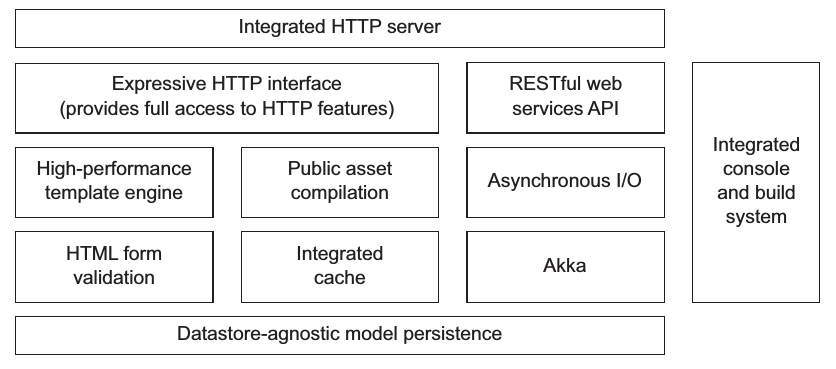
\includegraphics[width=0.8\textwidth, totalheight=6cm]{play_stack}
	\caption{\textit{Play Framework Stack}}
	\label{f3.1}
\end{figure}
\textbf{Play Framework Key Features Overview\cite{11}}
\begin{itemize}\itemsep1pt \parskip0pt \parsep0pt
\item Declarative application URL scheme configuration
\item Type-safe mapping from HTTP to Scala API
\item Type-safe templates
\item Embraces HTML5
\item Live code changes when you reload the page in your web browser
\item Full-stack framework (\cref{f3.1}), including persistence, security and internationalization
\end{itemize}
\textbf{Play versus Java EE}
\begin{figure}[!ht]
	\centering
		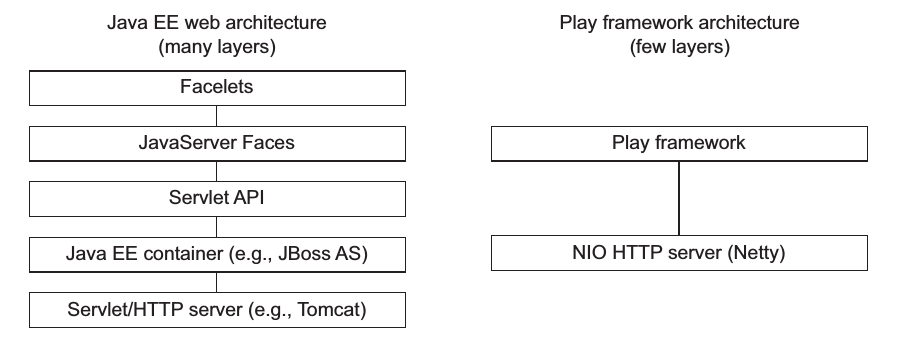
\includegraphics[width=0.8\textwidth, totalheight=6cm]{play_vs_java_ee}
	\caption{\textit{Java EE 'lasagna' architecture versus Play architecture}}
	\label{f3.2}
\end{figure}
From \cref{f3.2} is apparent how the framework embraces the simplicity in comparison with layered Java Enterprise Edition architecture. Whole framework stack is build on top of Netty\cite{19} client-server framework and doesn't require an application server container. Netty assures high performance of the stack and simple deployment of the application. Play has both, Java and Scala APIs (Application-Programming Interface) which will allow me use functional programming with Scala. I will discuss the framework in more depth in Back End Desing \cref{3.8} and Implementation \cref{4}.\par
\textbf{SDLC - Prototyping Model}\par
As discussed in Proposed Methodologies for The Web Application Development \cref{1.6.2}, I will use Prototyping Software Development Life-Cycle Model to develop the web application. Each step in development cycle is already listed and explained in Work Breakdown Structure \cref{1.7} of Project Plan.
\section{Proposed Tools}\label{3.3}
\subsection{Hardware}\label{3.3.1}
The project will be developed on DELL Latitude E5540 laptop machine lent to me by School of Computer Science, UCD where I work part-time as a research assistant. The laptop has following specification and should be sufficient to support this project development.
\begin{itemize}\itemsep1pt \parskip0pt \parsep0pt
\item \textbf{Procesor:} Intel Core i5-4310 CPU 2.00GHz x 4
\item \textbf{Memory:} 8GB RAM
\item \textbf{Graphics:} Intel Haswell Mobile
\item \textbf{Hard Disk:} 463 GB
\end{itemize}
\subsection{Software}\label{3.3.2}
I decided to use an open source, or at least free software tools. The thesis report will be written in LaTeX instead of an office suite.  Learning material will be written using the Markdown format, which require just a simple text editor. For the web application development I will need Java and Scala Development Kits with an IDE Studio. Additional tools will be needed to draw diagrams, take and edit screen shots, CSS, JSON or XML parsers and validation tools. For that I can utilize the operating system tools or online tools.
\begin{itemize}\itemsep1pt \parskip0pt \parsep0pt
\item \textbf{Operating System:} Ubuntu 14.04 LTS 64-bit\cite{21}
\item \textbf{Word Processing:} LaTeX suite witt Gummi simple LaTeX editor\cite{22}
\item \textbf{Markdown editor:} Remarkable\cite{23}
\item \textbf{IDE:} IntelliJ IDEA\cite{24}
\item \textbf{Web Development Framework:} Play Framework 2.4\cite{28}
\item \textbf{Distributed revision control system:} Git\cite{25}
\end{itemize}
\subsection{Deployment}\label{3.3.3}
Play Framework has very good deployment model. The application doesn't require a Java application server container, which greatly simplifies the deployment process in comparison to Java EE applications. There are various deployment options available, for example the application can be deployed as a standalone package and just copied to the deployment machine. Some of the cloud providers have built-in support for Play application deployment. Additional dependencies are handled by Simple Build Tool (SBT)\cite{29} which is included with the framework. For example,	 during the development, the framework is utilizing memory H2 database, but for the deployment the database management system can be replaced with MySQL for example. All need to be done is to edit the web application configuration file and SBT will handle the rest automatically.
\begin{itemize}\itemsep1pt \parskip0pt \parsep0pt
\item \textbf{Heroku:} The Heroku Cedar stack natively supports Play framework applications. A Postgres database is automatically provisioned for Play framework applications.\cite{26}
\item \textbf{Azure:} Microsoft Azure Cloud supports Play applications deployment on a web server with \emph{Azure Toolkit for Eclipse}. Another option is to dedicate a Vitual Machine (VM) to the application. Azure has numerous Linux images available, Ubuntu Server 14.04 included. The deployment should be then a simple question of moving the packaged application to the VM after all the required technologies are installed on the VM, such as Java and Scala runtime and database server.\cite{27}
\end{itemize}
\section{Web Application Content Design}\label{3.4}
In preparation for learning material writing, I collected some of the guidelines and recommendations of ways to structure the learning content with some tips on the writing style. Following material is only a short extract from the research conducted on numerous online resources dedicated to e-learning.
\subsection{The Lecture Structure}\label{3.4.1}
\begin{itemize}\itemsep1pt \parskip0pt \parsep0pt
\item \textbf{Introduction}
	\begin{itemize}\itemsep1pt \parskip0pt \parsep0pt
	\item Title
	\item Lecture content list
	\item Requirements (previous work or expected level of knowledge)
	\item Learning outcome
	\item Expected time requirements
	\end{itemize}
\item \textbf{Ending}
	\begin{itemize}\itemsep1pt \parskip0pt \parsep0pt
	\item Summary of main points
	\item Optional extra work
	\end{itemize}
\item \textbf{Signposts}
	\begin{itemize}\itemsep1pt \parskip0pt \parsep0pt
	\item Route the lecture by headings, which are related to objectives and emphasize the the structure of the lecture
	\item Indicate beginning and ending
	\item Emphasize important points
	\item Show relationships within the subject matter
	\end{itemize}
\end{itemize}
\subsection{Writing Style Tips}\label{3.4.2}
\begin{itemize}\itemsep1pt \parskip0pt \parsep0pt
\item Keep it simple
\item Keep it short
\item The 20 words per sentence is the maximum
\item 5 - 7 lines per paragraph
\item Maintain the variety in the writing style
\item Use positive rather than negative expressions
\item Use visuals and examples often
\end{itemize}

\section{Use Cases}\label{3.5}
\subsection{Prototype 1.0}\label{3.5.1}
\subsubsection{Prototype 1.0: Login Use Case}\label{3.5.1.1}

\begin{enumerate}
\item User logs in.
    \begin{enumerate}
    \item User reads the lectures.
    \item User adjusts the account settings.
     	\begin{enumerate}
     	\item User resets password.
     		\begin{enumerate}
     		\item User confirms password reset in email.
     		\end{enumerate}
     	\item User changes the address.
     	\end{enumerate}
   \end{enumerate}
\item User logs out.
\item User registers the account
   	\begin{enumerate}
    \item User validates the account in email.
   	\end{enumerate}
\end{enumerate}

\begin{figure}[!ht]
	\centering
		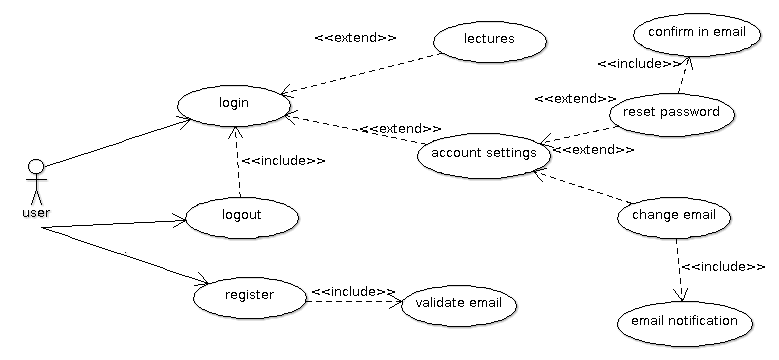
\includegraphics[width=0.7\textwidth, totalheight=5cm]{login_use_case}
	\caption{\textit{Prototype 1.0: Login Use Case}}
	\label{f3.5.1.1}
\end{figure}

\section{Sequence Diagrams}\label{3.6}
\subsection{Prototype 1.0}\label{3.6.1}
\subsubsection{Register Sequence Diagram}\label{3.6.1.1}
\begin{figure}[!ht]
	\centering
		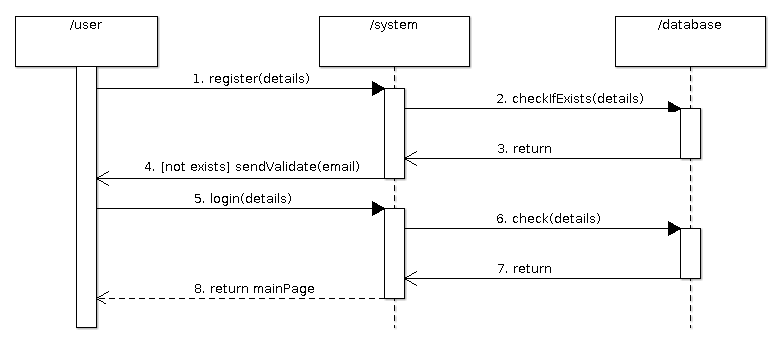
\includegraphics[width=0.8\textwidth, totalheight=5.5cm]{register_sequence_diagram}
	\caption{\textit{Prototype 1.0: Register Sequence Diagram}}
	\label{f3.6.1.1}
\end{figure}

\subsubsection{Account Settings Sequence Diagram}\label{3.6.1.2}
\begin{figure}[!ht]
	\centering
		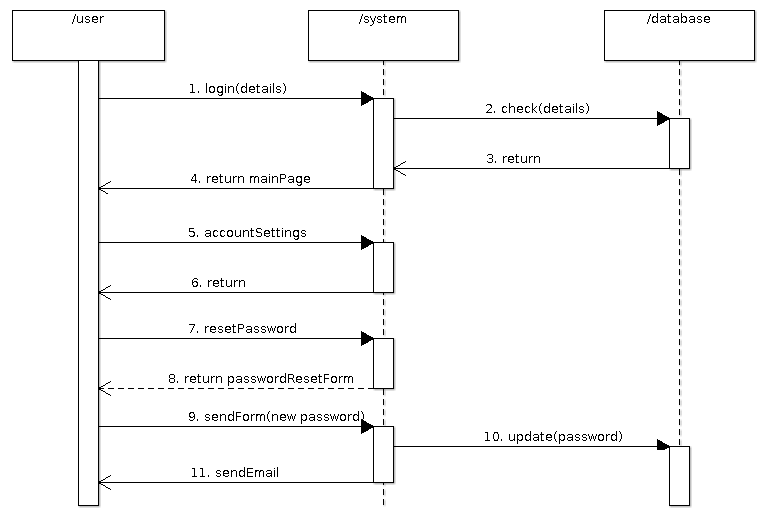
\includegraphics[width=0.8\textwidth, totalheight=6cm]{account_settings_sequence_diagram}
	\caption{\textit{Prototype 1.0: Account Settings Sequence Diagram}}
	\label{f3.6.1.2}
\end{figure}

\section{User Interface Design}\label{3.7}
\subsection{Prototype 1.0}\label{3.7.1}
\subsubsection{Main Page Wireframe}\label{3.7.1.1}
\begin{figure}[!ht]
	\centering
		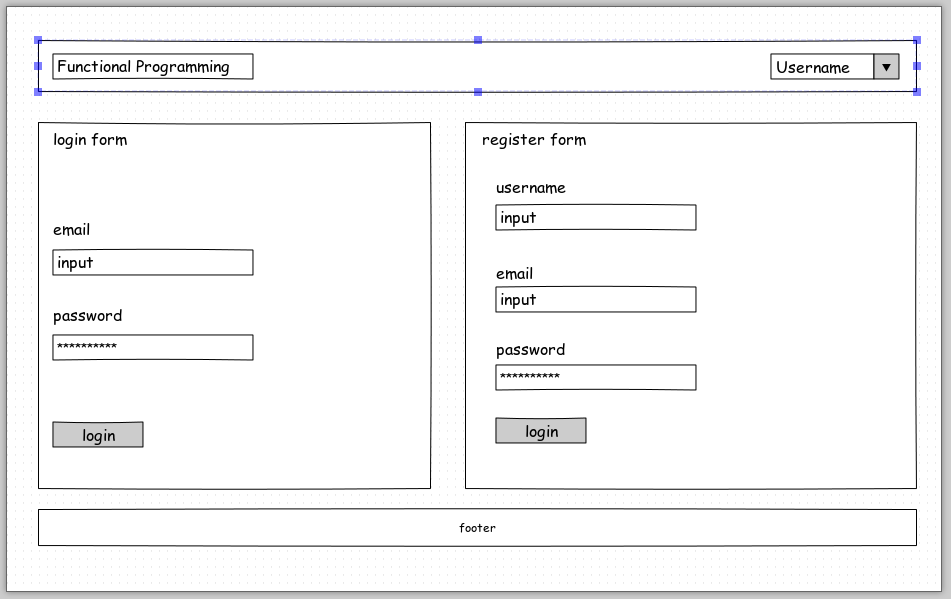
\includegraphics[width=0.9\textwidth, totalheight=7cm]
		{wireframe_main_page}
	\caption{\textit{Prototype 1.0: Main Page Wireframe}}
	\label{f3.7.1.1}
\end{figure}

On the main page, the user can log-in or register a new account. If the user attempts to log-in without the account, the attempt is rejected. The successful log-in will result in redirection to the dashboard page. Upon successful account registration, the user will receive the email with a confirmation link which he must click to validate the registration.

\textbf{Required Elements}
\begin{itemize}
\item header (label, hidden drop-down menu)
\item login form (labels, text input, password input, button)
\item register form (4 labels, text inputs, password input, button)
\item footer
\end{itemize}

\subsubsection{Dashboard Wireframe}\label{3.7.1.2}
\begin{figure}[!ht]
	\centering
		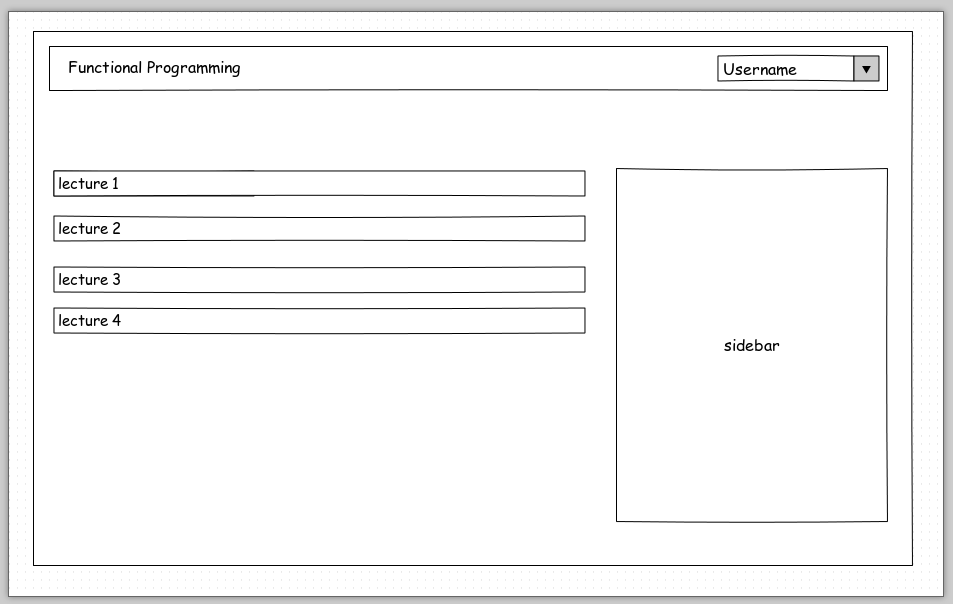
\includegraphics[width=0.9\textwidth, totalheight=7cm]
		{wireframe_dashboard}
	\caption{\textit{Prototype 1.0: Dashboard (lectures) Wireframe}}
	\label{f3.7.1.2}
\end{figure}

On the dashboard page user will have access to the lectures. Also, the drop-down menu in the header will be visible and will allow the user to request the account settings page or log-out. The account setting request will result in the account settings page redirection and the log-out request will result in the redirection to the main page.

\textbf{Required Elements}
\begin{itemize}
\item header (label, visible drop-down menu)
\item main area (links to the lectures)
\item side area (for future functionality)
\item footer
\end{itemize}

\subsubsection{Account Settings Wireframe}\label{3.7.1.3}
\begin{figure}[!ht]
	\centering
		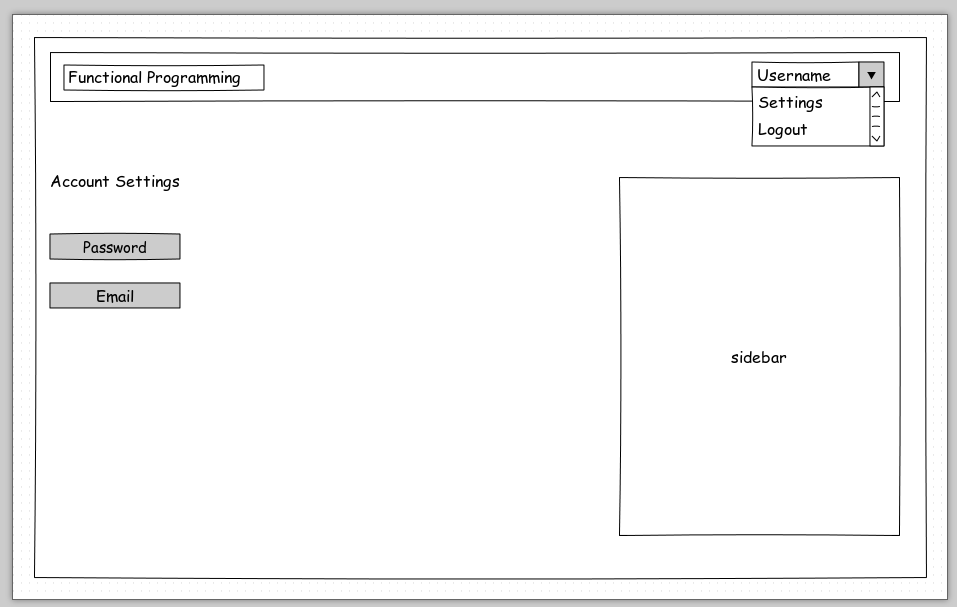
\includegraphics[width=0.9\textwidth, totalheight=7cm]
		{wireframe_account_settings}
	\caption{\textit{Prototype 1.0: Account Settings Wireframe}}
	\label{f3.7.1.3}
\end{figure}

On the account setting page, the user can change the password or the email address. Upon the password change request, the email will be sent to the user with the confirmation link. Upon the successful email change, the user will receive the notification email.

\textbf{Required Elements}
\begin{itemize}
\item header (label, visible drop-down menu)
\item main area (2 buttons)
\item side area (for future functionality)
\item footer
\end{itemize}

\section{Database Schema Design}\label{3.8}
\subsection{Prototype 1.0}\label{3.8.1}

For the prototype 1.0 functionality, I will need the entity which will represent the user and the entity which will represent a random token. I will generate a token and associate it with the user every time a user requests registration, password change or email change. These tokens will then be embedded into an URL which will be sent to user's email. It's basically a way of identifying the user actions. The user then must click the URL to validate (confirm) the action. There should be a general expiration period associated with each token. Let's say one day. If the user doesn't confirm the requested action the action will be cancelled. For this functionality, I will need to save the token creation time-stamp as well.

\begin{figure}[!ht]
	\centering
		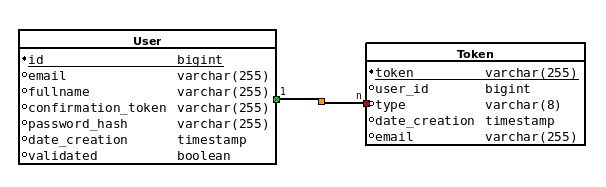
\includegraphics[width=0.6\textwidth, totalheight=4.5cm]
		{entity_relations_diagram1}
	\caption{\textit{Prototype 1.0: Entity Relations Diagram}}
	\label{f3.8.1}
\end{figure}

\section{Back End Design}\label{3.9}
\subsection{Prototype 1.0}\label{3.9.1}
In Play! Framework the user interfaces are represented by views. The view consists of HTML, Javascript and embedded Scala\cite{30} code. The views are compiled to Scala classes and stored in /views folder. The views are rendered on demand by the server.

The user interacting with the views creates the requests to the resources. The incoming requests are handled by controllers. Each request is routed to the one controller method. Controller methods are processing the request and returning responses which in turn render the views. Controllers are stored in /controllers folder.

The requests are routed to the controllers by rules stored in /conf/routes file. In this file, the mappings form URIs to controller methods are defined. Play Framework uses REST like approach to routing. The /conf directory serves as a storage for all configuration files.

\begin{figure}[!ht]
	\centering
		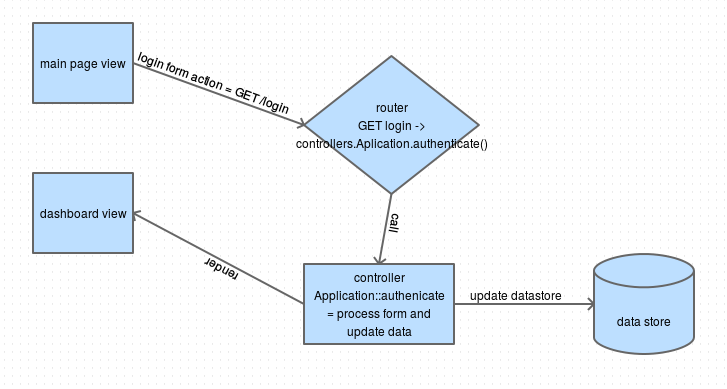
\includegraphics[width=0.8\textwidth, totalheight=7cm]
		{play_flowchart}
	\caption{\textit{View -> Request -> Controller -> Response -> View Diagram}}
	\label{f3.9.2}
\end{figure}

Play Framework is persistence agnostic, but it provides Java Ebeans ER mapper and H2 in memory database by default. H2 can be changed for other database implementation for the production mode and any other ER mapping framework can used instead of Ebeans. In Ebeans, the each entity is represented by a POJO annotated class called model. Models are stored in /models directory.

The layout of a Play application is standardized to keep things as simple as possible. After a first successful compile, a Play application looks like this:

\begin{figure}[!ht]
	\centering
		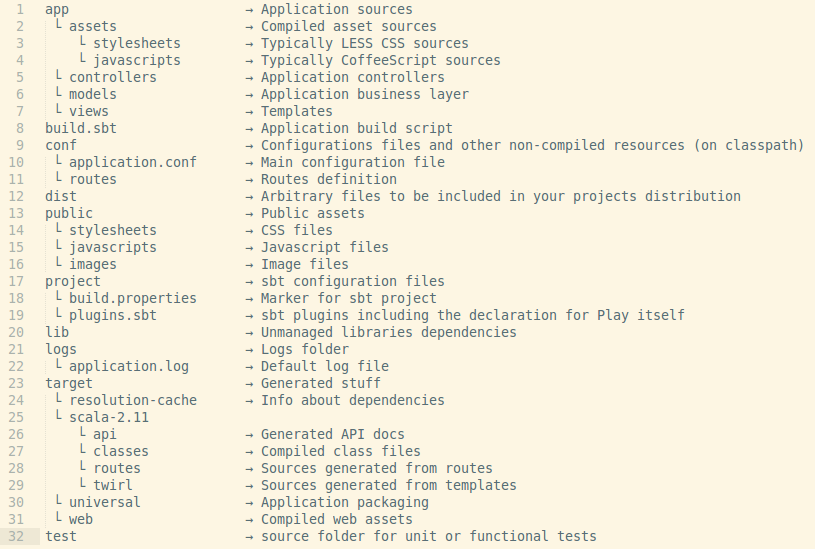
\includegraphics[width=1\textwidth, totalheight=10cm]
		{play_framework_project_anatomy}
	\caption{\textit{Play Framework Project Anatomy}}
	\label{f3.9.1}
\end{figure}

\section{Project Repository Design}\label{3.10}
Project repository will be hosted on GitHub page: \url{https://github.com/zubidlo/itb_honours_project}.
I propose following directory structure:

\begin{figure}[!ht]
	\centering
		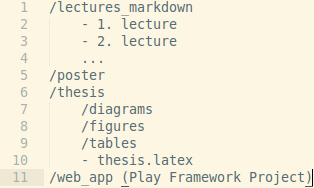
\includegraphics[width=0.4\textwidth, totalheight=4cm]
		{github_repo_anatomy}
	\caption{\textit{GitHub Repository Anatomy}}
	\label{f3.10}
\end{figure}

\section{Conclusion}\label{3.11}
It this section I discussed the preliminary design of the project. I argued that the prototyping software development methodology would the appropriate approach in the development of this project. I outlined the form the learning material should take and I decided to use Scala programming language to communicate functional programming ideas in code.

The web application publishing the learning material for students will be developed using Play! Framework. The application design will follow the standardized anatomy of a Play application and I will use Git as versioning system and GitHub repository to store the project. Play supports both Java and Scala programming languages and I have not yet decided what programming language I will use to develop the application. Also, I listed all the tools I will use in the project implementation.

With the help of UML, I outlined proposed design for web application prototype version 1.0. In this prototype iteration, the application will support user log-in and registration, account settings and log-out. The application will require email validation with expiration date and password should be stored as encrypted hashes. The application will also list all the learning material and reserve a space for an additional functionality.
%_______________________________chapter_______________________________________
\chapter{Implementation}\label{4}
\section{Introduction}\label{4.1}
In this section, I will discuss some of the web application implementation details. As outlined in chapter \ref{3.9.1} the application will be rendered on the server side and will consist of views, routes, controllers, and models. The views are basically HTML pages returned by the server on user requests. They are all the user is seeing and interacting with.

\begin{figure}[!ht]
	\centering
		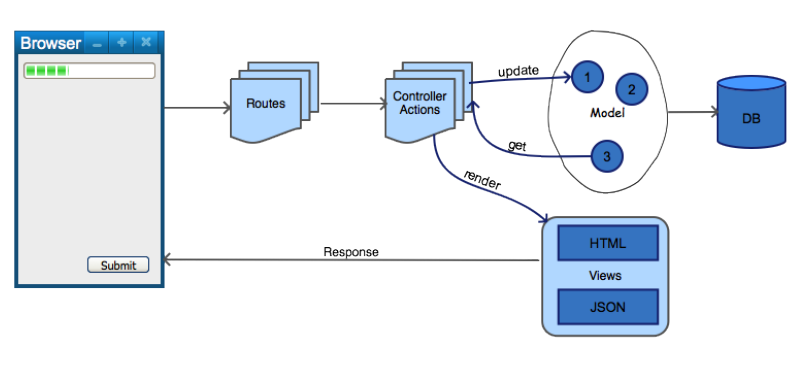
\includegraphics[width=0.7\textwidth, totalheight=5.8cm]
		{play_workflow_diagram}
	\caption{\textit{Play WorkFlow Diagram}}
	\label{f4.1}
\end{figure}

The rest of the Play infrastructure is working in "the background" to make sure that views are returned to user filled with appropriate data. The router routes the requests such as an HTML form POST action to a controller method which will process the form. For example, log-in form POST request will be routed to the appropriate controller method, which will first validate the form. Next, the user data will be fetched from the model and compare to the data in the form. If there is a match, the controller method will render the dashboard view and send it back to the user. Also, the server will maintain the session during the user interaction with the views as long as the user is logged-in.

The application will be developed locally on a laptop and deployed on a live internet server. I chose Microsoft Azure Cloud for the deployment.  The reason is that I already have the access to the Azure and I'm familiar with the service management console.

\section{Development Set-Up}\label{4.2}
The Play Framework is the part of Lightbend Reactive Platform\cite{32}. The platform uses Lightbend Activator User Interface for the development. The user installs the activator locally and starts the service. The user interface is spawned in the browser (figure \ref{f4.2}) in which user can create new web application or develop, build, run and test existing web application. I used activator and eclipse for the application development.

The new application development doesn't start from scratch, but user rather creates a new application by choosing one of 400 templates. These templates are scaffolds consisting of standardized Play project directory structure and already imported libraries required for chosen type of the web application. Also, the templates serve the role of tutorials for the beginners, which is very useful to me. I created the new Play Java application from a template tutorial showcasing the user log-in and I imported additional Javascript libraries for user interface enhancement such as Scala code highlighting.

\begin{figure}[!ht]
	\centering
		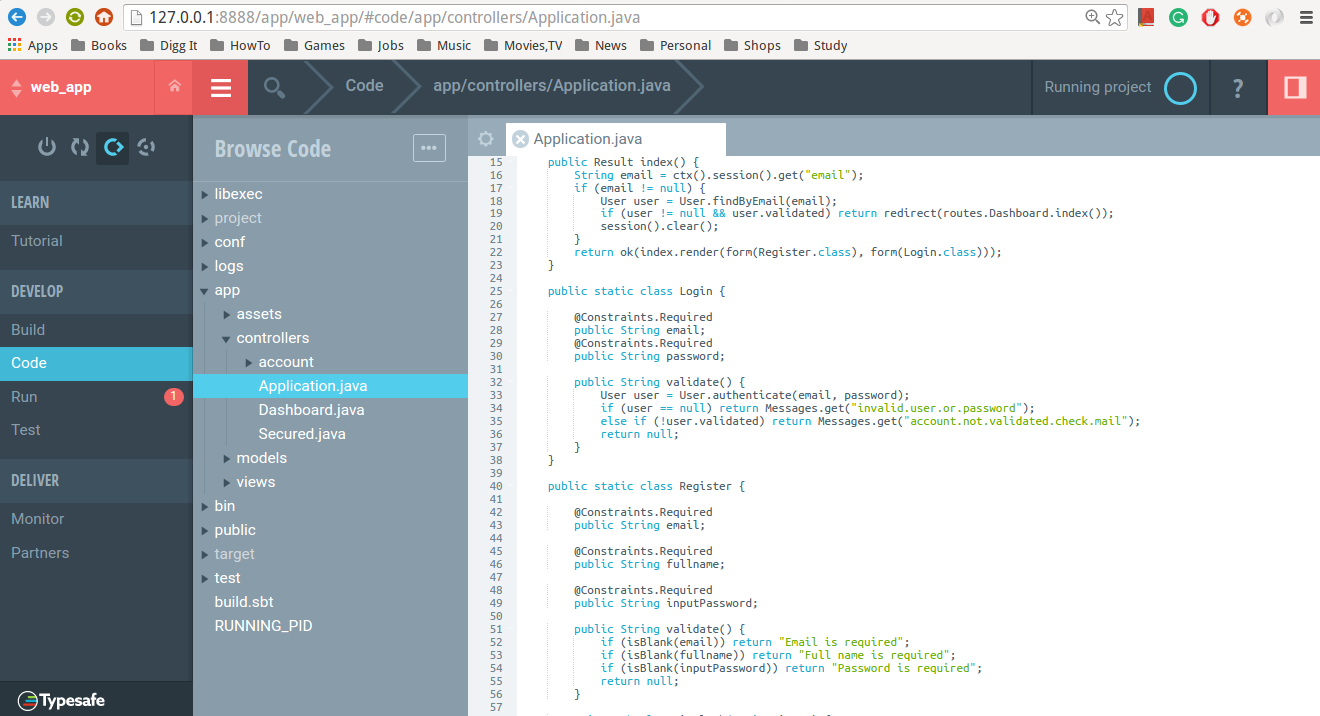
\includegraphics[width=0.9\textwidth, totalheight=8cm]
		{activator}
	\caption{\textit{Lightbend Activator}}
	\label{f4.2}
\end{figure}

\section{User Interfaces (Views)}\label{4.3}
The views are developed with usage of Scala templates. Each view is compiled to the Scala object and the HTML can be then rendered by calling the render() method on the given view object. This action is usually done in a controller method as the last step before the rendered HTML is inserted in the response. The view can be arbitrary nested, allowing for creating common layouts (header, footer) just once. The views can carry state-full information as well, such as references to some useful values existing outside the views. This can be used to maintain the session state for example. Every view must have a reference to a user object, which gets created when a user successfully logs in. In the case the user object is not available, a view will redirect to the index page. This way only the logged-in user would get an access to certain views.

\subsection{Prototype 1.0}\label{4.3.1}
\subsubsection{Main Layout View}\label{4.3.1.1}
The main layout view consists of a header (navigation bar) and footer. References to the User and additional HTML @content are imported at the top of the view. Every additional view is then inserted on @content placeholder. Also, scripts and CSS are imported in this view.
\begin{figure}[!ht]
	\centering
		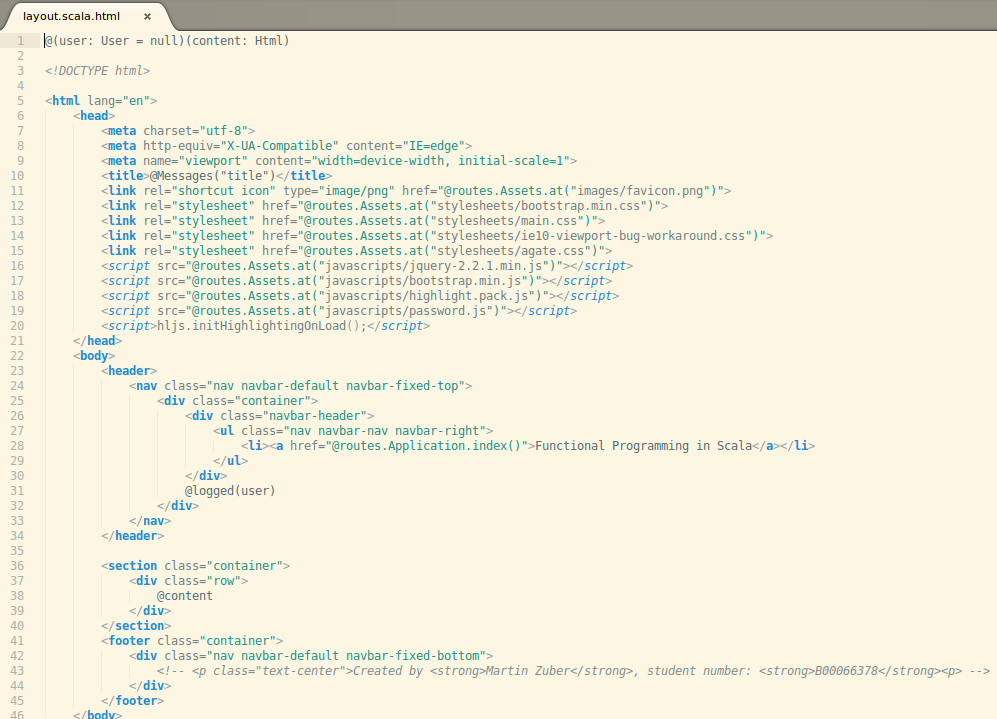
\includegraphics[width=0.9\textwidth, totalheight=8cm]
		{main_layout_view}
	\caption{\textit{Main Layout View}}
	\label{f4.3.1.1}
\end{figure}

\subsubsection{Index View}\label{4.3.1.2}
The index view consists of 2 forms, the login and register form. The view is inserted into main layout view and rendered by the server as the main page of the web application.

\begin{figure}[!ht]
	\centering
		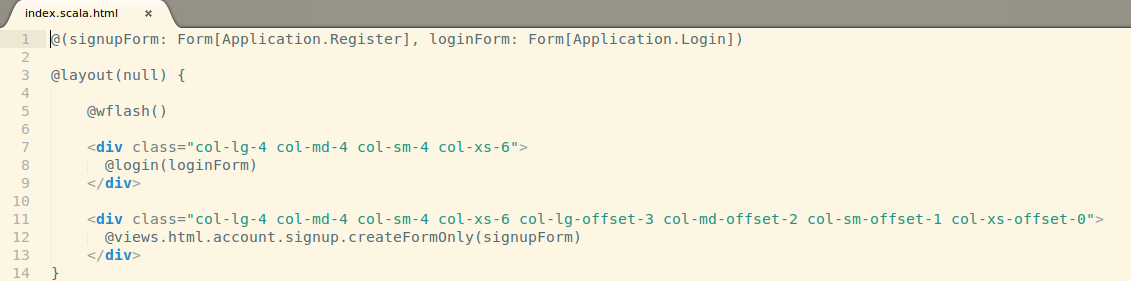
\includegraphics[width=0.9\textwidth, totalheight=4cm]
		{index_view}
	\caption{\textit{Index View}}
	\label{f4.3.1.2}
\end{figure}

The figure \ref{f4.3.1.3} is a snapshot of the rendered main page.

\begin{figure}[!ht]
	\centering
		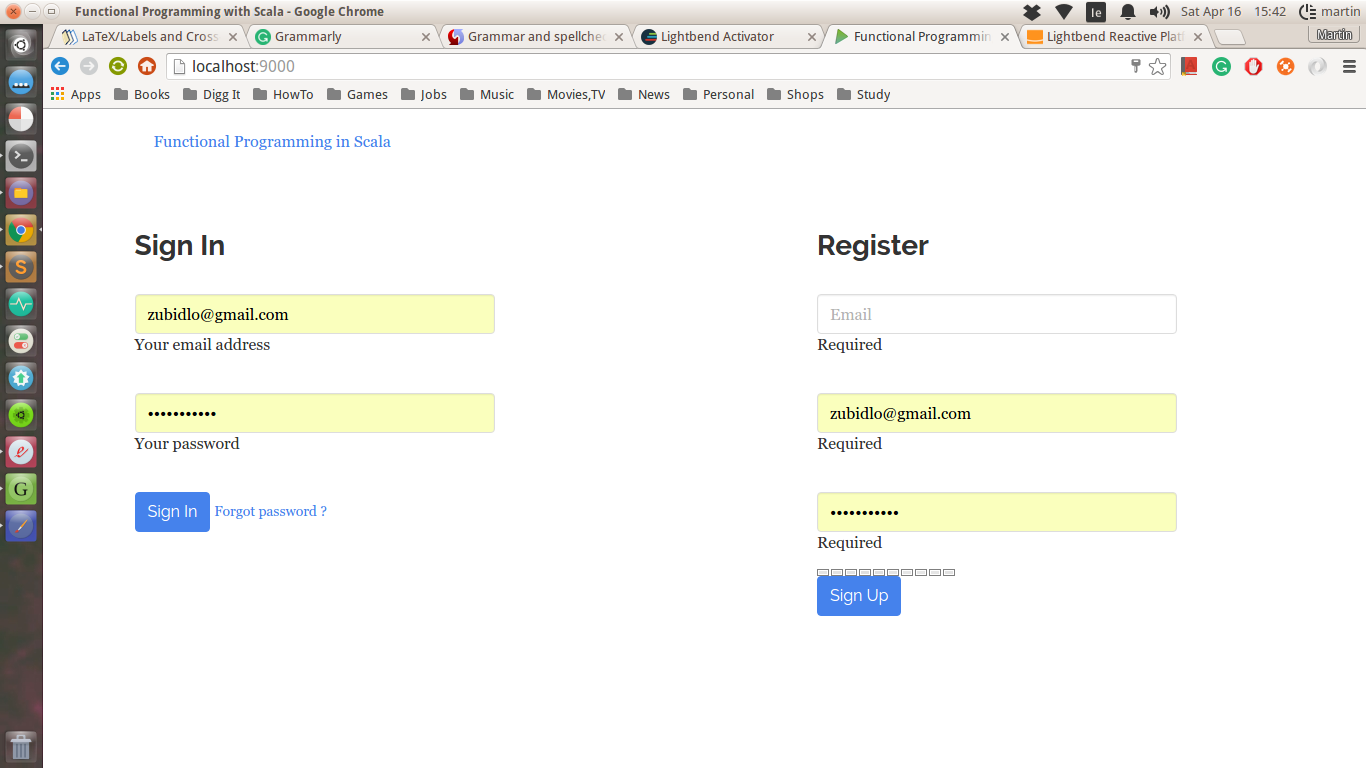
\includegraphics[width=0.89\textwidth, totalheight=8cm]
		{main_page_view}
	\caption{\textit{Main Page}}
	\label{f4.3.1.3}
\end{figure}

All the user interface implementations in Prototype 1.0 are following this pattern. The layout view is a container in which appropriate views are inserted on required places. This nested structure is then turned into HTML and added to the HTML response.

\section{Data Models}\label{4.4}
\subsection{Prototype 1.0}\label{4.4.1}
//TODO

\section{Business Logic (Controllers)}\label{4.5}
\subsection{Prototype 1.0}\label{4.5.1}
//TODO

\section{Deployment Set-Up}\label{4.6}
//TODO

\section{Conclusion}\label{4.7}
//TODO

%_______________________________chapter_______________________________________
\chapter{Testing and Evaluation}\label{5}
\section{Introduction}\label{5.1}
//TODO

\section{User Interface Tests}\label{5.3}
//TODO

\section{Unit Tests}\label{5.2}
//TODO

\section{Conclusion}\label{5.4}
//TODO

%_______________________________chapter_______________________________________
\chapter{Conclusion and Further Work}\label{6}

\section{Introduction}\label{6.1}
//TODO

\section{Achievements}\label{6.2}
//TODO

\section{Personal Gain}\label{6.3}
//TODO

\section{Further Work}\label{6.4}
//TODO

\section{Conclusion}\label{6.5}
//TODO

%_______________________________Bibliography_______________________________________
\addcontentsline{toc}{section}{Bibliography}
\bibliographystyle{plain}
\setstretch{1}
\begin{thebibliography}{99}

\bibitem{1}
Neil Ford,
\emph{Functional thinking: Why functional programming is on the rise},
\url{http://www.ibm.com/developerworks/library/j-ft20/},
(2013-01-25)

\bibitem{2}
Typesafe,
\emph{Scala, Object-Oriented Meets Functional},
\url{http://www.scala-lang.org/},
(2002-2015)
	
\bibitem{3}
Typesafe,
\emph{Scala in the Enterprise},
\url{http://www.scala-lang.org/old/node/1658},
(2012-01-19)

\bibitem{4}
Brikman, Yevgeniy,
\emph{The Play Framework at LinkedIn: Productivity and Performance at Scale},\\
\url{https://www.youtube.com/watch?v=8z3h4Uv9YbE&ab_channel=NewCircleTraining},
(2013-06-26)

\bibitem{5}
Wampler, Dean,
\emph{We Won! How Scala Conquered the Big Data World.},
\url{https://www.youtube.com/watch?v=AHB6aJyhDSQ&ab_channel=NewCircleTraining},
(2015-03-01)

\bibitem{6}
theotown,
\emph{Akka wins 2015 JAX Award for Most Innovative Open Source Technology},
\url{https://www.typesafe.com/blog/akka-wins-2015-jax-award-for-most-innovative-open-technology},
(2015-03-23)
	
\bibitem{7}
Wikipedia,
\emph{Free software programmed in Scala},
\url{https://en.wikipedia.org/wiki/Category:Free_software_programmed_in_Scala},
(2015-01-05)
	
\bibitem{8}
Wikipedia,
\emph{Play Framework},
\url{https://en.wikipedia.org/wiki/Play_framework},
(2015-10-04)
	
\bibitem{9}
Paul Chiusano,	Runar Bjarnason,
\emph{Functional Programming in Scala.},
Shelter Island, NY 11964,
Manning Publications Co., 2015. ISBN 9781617290657.

\bibitem{10}
Dean Wampler, Alex Payne,
\emph{Programming Scala, Second Edition.},
1005 Gravenstein Highway North, Sebastopol, CA 95472,
O’Reilly Media, Inc., 2015. ISBN: 978-1-491-94985-6.
	
\bibitem{11}
Peter Hilton, Erik Bakker, Francisco Canedo,
\emph{Play For Scala.},
Shelter Island, NY 11964,
Manning Publications Co., 2014. ISBN 9781617290794.

\bibitem{12}
Hudak, P.,
\emph{The Conception, Evolution, and Application of Functional Programming Languages.},
s.l.:Yale University Department of Computer Science,
1989

\bibitem{13}
Hristakeva, M., Vuppala, R.,
\emph{A Survey of Object Oriented Programming Languages.},
Santa Cruz: Univ. of California.
2009

\bibitem{14}
Hughes, J.,
\emph{Why Functional Programming Matters.},
Goteborg Institutionen for Datavetenskap,
Chalmers Tekniska Hogskola, 1984


\bibitem{15}
Goyri, A., Franklin, L., Dig, D., Lahoda, J.,
\emph{Crossing the Gap from Imperative to Functional, Programming through Refactoring.},
Saint Petersburg: s.n.,
2013

\bibitem{16}
Roy, P. V.,
\emph{Programming Paradigms for Dummies: What Every Programmer Should Know.},
s.l.:IRCAM/Delatour,
2009

\bibitem{17}
Odersky M., Altherr P., Cremet V., Dragos I., Dubochet G.,
\emph{An Overview of the Scala Programming Language},
s.l.:IRCAM/Delatour,
Second Edition,
2006

\bibitem{18}
Wikipedia,
\emph{Read-Eval-Print Loop},
\url{https://en.wikipedia.org/wiki/Read-eval-print_loop},
(2015-11-21)

\bibitem{19}
Netty is an asynchronous event-driven network application framework ...,
\emph{Netty Project},
\url{http://netty.io/},
2016

\bibitem{20}
Markdown,
\emph{Daring Fireball},
\url{https://daringfireball.net/projects/markdown/	},
2002-2016

\bibitem{21}
Ubuntu 14.04.3 LTS,
\emph{Canonical Ltd.},
\url{http://www.ubuntu.com/download/desktop}
2016

\bibitem{22}
Gummi, The Simple LaTeX editor,
\emph{alexandervdm},
\url{https://github.com/alexandervdm/gummi},
2016

\bibitem{23}
Remarkable,
\emph{Jamie McGowan},
\url{http://remarkableapp.github.io/},
2015

\bibitem{24}
Intellij IDEA,
\emph{JetBrains s.r.o},
\url{https://www.jetbrains.com/idea/},
2000-2016

\bibitem{25}
Git,
\emph{Linus Torvalds, Software Freedom Conservancy},
\url{https://git-scm.com/},
2005-2016

\bibitem{26}
Heroku Play Framework Support,
\emph{Heroku.com},
\url{https://devcenter.heroku.com/articles/play-support},
2016-01-22

\bibitem{27}
Deploying Play Framework Apps with the Azure Toolkit for Eclipse,
\emph{Kirk Evans[MSFT]},
\url{https://blogs.msdn.microsoft.com/kaevans/2015/05/12/deploying-play-framework-apps-with-the-azure-toolkit-for-eclipse/},
2015-05-12

\bibitem{28}
The High Velocity Web Framework For Java and Scala,
\emph{Typesafe},
\url{https://www.playframework.com},
2016

\bibitem{29}
The Interactive Build Tool,
\emph{Typesafe},
\url{http://www.scala-sbt.org/},
2015

\bibitem{30}
Scala Twirl Engine,
\emph{Play Framework},
\url{https://github.com/playframework/twirl},
2016

\bibitem{31}
Ebean ORM for Java/Kotlin,
\emph{Avaje},
\url{http://ebean-orm.github.io/},
2016

\bibitem{32}
LightBend Reactive Platform,
\emph{Typesafe},
\url{https://www.lightbend.com/products/lightbend-reactive-platform},
2016

\end{thebibliography}

%_______________________________appendix_______________________________________
\appendix
\chapter{The Learning Material}\label{A}
\section{Functional Programming with Scala}\label{A.2}
\subsection{Preface}\label{A.3}
As a Computer Science student at ITB, I was introduced to computer programming through Java programming language. First, we learned the syntax of the language. Next, we have been introduced to the object-oriented approach to designing software and how to work with libraries such as Swing. Later in the third year, we learned the basics of concurrency and some design patterns for solving reoccurring problems. Around this time I crossed the initial steep part of the programming learning curve and I was comfortable enough with Java to learn some additional language features and Java Standard Edition platform libraries. Programming with Java became my hobby and I found a time to read additional material such as "Thinking in Java" from Bruce Eckel or "Effective Java" from Joshua Bloch.\par
At the same time, Oracle introduced important update number 8 to Java platform which, among other things introduced the syntax for anonymous functions (lambdas) and a number of libraries dedicated to functional programming style, such as Stream API. I was interested in this new functionality and started to learn to implement these tools and ideas into my code. Playing with lambdas, streams, and optionals I started to realize the power and elegance behind and I got really curious about the theory behind the functional programming.\par
Any student trying to learn about functional programming within JVM ecosystem will very soon become aware of programming language called Scala. The reason is that Scala has by design more richer support for functional programming than Java and hence is better suited as a vehicle for the study. At some point of the study one will become familiar with other programming languages such as Haskell or ML. There are various reasons for this, main being that these language's syntax is designed to emphasize the functional programming ideas.\par
The following material is an overview of what I learned about functional programming in the period of 2 semesters in time dedicated to honors degree final project and my own spare time. I used Scala syntax to communicate ideas with code.

\subsection{Pure vs Impure Functions}\label{A.4}
Well, functional programming is a programming style where programs are constructed using only \emph{pure functions}. What are these pure functions you may ask? 

Well, pure function is any function with following properties:
\begin{enumerate}
\item The function \emph{always} evaluates to the same result given the same argument. The word always is emphasized here. The pure function can return the same result for different arguments, but it can never return different results for the same argument.
\item Evaluation of the result does not cause any semantically observable \emph{side effect}. Well, what are these side effects then? In Computer Science, a function or expression is said to have a side effect if it modifies some state or has an interaction with calling functions or the outside world. Basically, a function has a side effect if it does something else than returning a result. Some examples of side effects:
\begin{itemize}
\item Modifying a variable or a data structure in place
\item Throwing an exception or halting with an error
\item Writing to or reading from the console or a file
\item Drawing on the screen, updating a database, printing on a printer
\end{itemize}
\end{enumerate}

\textbf{Example: Common Pure and Impure Functions}

\begin{lstlisting}
 sin(x)
 length(list)
 random(seed)
 printf(string)
\end{lstlisting}

Functions \emph{sin(x)} and \emph{length(list)} are pure functions because they always return the same result for the same argument and do nothing else. Function sin(0) is always 0 and length of the same list is always the same result.\par
Functions \emph{random(seed)} and \emph{printf(string)} are impure functions because random(1) will not always return the same result. It will return a random number from 0 to 1. Function printf("hello world") will print the string literal to the console and return no result. Even that is not guaranteed. Sometimes it can throw an exception if the console is not available for example. Impure functions are called \emph{procedures} in computer science.

\textbf{Example: Function definitions in Scala}
\begin{lstlisting}
	def add1(a: Int, b: Int): Int = return a + b;
	def add2(a: Int, b: Int): Int = a + b
	def add3(a: Int, b: Int) = a + b
	val add4: (Int,Int) => Int = (a: Int, b: Int) => a + b
	val add5 = (a: Int, b: Int) => a + b
	def add6(a: Int)(b: Int) = a + b
	val add7 = Int => Int => Int = a => b => a + b
\end{lstlisting}

\begin{enumerate}
\item On line 1 is a function definition where I defined a function \emph{add1} which takes two arguments of type Int and returns Int result which is just the addition of the arguments.
\item \emph{add2} defines exactly same function without \emph{return} word and \emph{semicolon}
\item \emph{add3} is the same function with return type left out
\item Line 5 is not a function definition statement, but assignment to an  
immutable value named \emph{add4}. The value of an anonymous function described by \emph{(a: Int, b: Int) => a + b} was assigned to the name \emph{add4}. This form of function description is called a \emph{function literal} or a \emph{lambda expression}. It's the same function with emphasis on it's type: \emph{(Int, Int) => Int}. It's a type of a function which takes 2 Int arguments and returns Int result. 
\item \emph{add5} is again a value which holds a function literal. This time the type is omitted and the function is only expressed by the lambda expression.
\item \emph{add6} is again the same function defined in \emph{curried form}, which we will discuss later.
\item \emph{add7} is again the same function value, but with it's type \emph{Int => Int => Int} emphasizes the curried form and the fact that every function is a function which takes one argument and returns one result. We will discuss these ideas later as well.
\end{enumerate}

Here are the the function call statements where 4 and 5 were passed as arguments. All seven functions will return 9 as the result. 
\begin{lstlisting}
	add1(4,5); add2(4,5); add3(4,5); add4(4,5);	add5(4,5); 
	add6(4)(5);	add7(4)(5);
\end{lstlisting}

Here are some important points to realize:

\begin{itemize}
\item All seven functions represent the same function which adds two Int values and returns the result.
\item This function is a pure function because it always returns the same value 9 for the same arguments 4, 5 and doesn't do any side effects.
\item In Scala and functional programming in general, functions are values. The same way as objects are values. We can assign functions to variables, pass them as arguments to other functions, create them inside the functions and return them as results of function computations. Later we will see that as long as the functions are pure they hold other very useful characteristics we can utilize in our functional programs.
\item The functions can be expressed as literals. The same way we can create anonymous objects or a string literal "hello world", we can create a function literal in a form of a lambda expression.
\end{itemize}
\end{document}